\documentclass[11pt,a4paper]{article}
\usepackage[utf8]{inputenc}
\usepackage[english]{babel}
\usepackage[T1]{fontenc}
\usepackage{charter}
\usepackage{amsmath}
\usepackage{amsfonts}
\usepackage{amssymb}
\usepackage{esint}
\usepackage[table]{xcolor}
\usepackage{graphicx}
\usepackage[left=1.5cm,right=1.5cm,top=2cm,bottom=2cm]{geometry}
\usepackage{tikz}
\usepackage{tikz-3dplot}
\usetikzlibrary{babel}
\usepackage[font=small,labelfont={small,bf},margin=0.5cm,justification=justified]{caption}
\usepackage[font=small,labelfont={small,bf}]{subcaption}
\usepackage{epstopdf}
\usepackage{natbib}
\usepackage[nointegrals]{wasysym}
%\renewcommand\familydefault\sfdefault
\usepackage[italic,defaultmathsizes]{mathastext}
\usepackage{hyperref}
\usepackage{lipsum}
\usepackage{threeparttable}
\usepackage{titling}
\usepackage[bf]{titlesec}
\usepackage{abstract}
\usepackage{lastpage}
\usepackage{fancyhdr}
\usepackage{csvsimple}
\usepackage{longtable}
\usepackage{pdflscape}
\usepackage{authblk}
\usepackage{calculator}
\usepackage{multirow}

\hypersetup{
%      draft,
   linktocpage=true,
    colorlinks=true,
    linkcolor=blue,
    citecolor=blue,
    filecolor=blue,      
    urlcolor=blue
}

\tikzset{>=latex}
\usetikzlibrary{arrows}
\pgfarrowsdeclarecombine{latexo}{latexo}
{*}{latex}{latex}{*}

%\numberwithin{equation}{section}
\renewcommand\Authfont{\large}
\renewcommand\Affilfont{\small}
%\renewcommand\abstractnamefont{\fontfamily{qcr}\selectfont}

\pretitle{\begin{center}\LARGE\bfseries}
\posttitle{\end{center}}

\titlelabel{\thetitle. \,}

\author[1,2]{Santiago H. Luna}

\affil[1]{Instituto de Estudios Andinos ``Don Pablo Groeber'' (\textsc{idean}). Universidad De Buenos Aires -- \textsc{conicet}.}
\affil[2]{Instituto de Tecnología e Ingeniería. Universidad Nacional de Hurlingham.}

\title{thermev2 -- A thermal model for the Earth} 

\date{\today}

\pagestyle{fancy}

\fancypagestyle{firststyle}
{
      \fancyhf{}
      \chead{\small{Manuscript -- File name: \textit{thermev2 doc} -- Version 1}}
      \lfoot{Corresponding author: Santiago Luna (\href{mailto:sluna@gl.fcen.uba.ar}{sluna@gl.fcen.uba.ar})}
      \rfoot{Page \thepage \ of \pageref{LastPage}}
      \renewcommand{\headrulewidth}{0.4pt}
      \renewcommand{\footrulewidth}{0.4pt}
}

\fancyhf{}
\lhead{\small{thermev2 -- A thermal model for the Earth}}
\rhead{\small{Luna, S.H.}}
\cfoot{Page \thepage \ of \pageref{LastPage}}
\renewcommand{\headrulewidth}{0.4pt}
\renewcommand{\footrulewidth}{0.4pt}

\newcommand{\sgn}{\mathop{\text{sgn}}}
\newcommand{\apj}{The Astrophysical Journal}
\newcommand{\diff}[0]{\text{d}}
\newcommand{\fdiff}[2]{\frac{\text{d} #1}{\text{d} #2}}
\newcommand{\pdiff}[2]{\frac{\partial #1}{\partial #2}}
\newcommand{\fddiff}[2]{\frac{\text{d^2} #1}{\text{d} #2^2}}
\newcommand{\degr}[0]{^{\circ}}
\newcommand{\chel}[4]{^{#1}_{#2}\text{#3}^{#4}}
\newcommand{\valmed}[1]{\left\langle #1 \right\rangle}
\newcommand{\E}[1]{\times 10^{#1}}
\renewcommand{\vec}[1]{\mathbf{#1}}
\newcommand{\vecg}[1]{\boldsymbol{#1}}
\newcommand{\iu}{\text{i}}
\newcommand{\norm}[1]{\left\vert\left\vert #1 \right\vert\right\vert}
\newcommand{\abs}[1]{\left\vert #1 \right\vert}
\renewcommand{\arraystretch}{1.5}
\newcommand{\apendice}{
      \appendix\numberwithin{equation}{section}
      \titleformat{\section}{\Large\bfseries}{\appendixname \ \thesection .}{0.35em}{}
      \titleformat{\subsection}{\large\bfseries}{\thesubsection .}{0.35em}{}
      \titleformat{\subsubsection}{\normalsize\bfseries}{\thesubsubsection .}{0.35em}{}
}

\tdplotsetmaincoords{70}{110}

\begin{document}

\maketitle

\thispagestyle{firststyle}

\section{Introduction\label{sec:intro}}

This document provides a description of a model to simulate the thermal evolution of the Earth's interior, that is, the time evolution of the characteristic temperatures of the mantle and core of the Earth throughout its history, which is mainly based on the models developed by \citet{stevensonetal1983} and \citep{tosietal2017} including the heat generated by tidal interaction.

The earth is considered to be divided into two parts: the core and the mantle (see Fig.~\ref{fig:Earth_interior}). Both are bounded by two concentric spherical surfaces, an outer one of radius $R_\oplus$, which is the mean radius of the Earth, and the inner one of radius $R_\text{c}$, which is equal to the radius of the core. The latter defines the core-mantle boundary (CMB).

\begin{figure*}[t]
      \centering
      \begin{subfigure}[b]{0.45\textwidth}
      \centering
      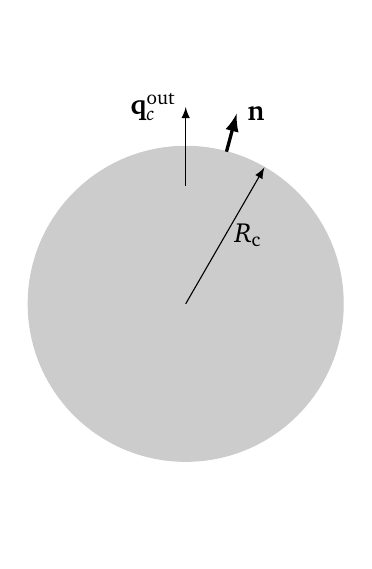
\begin{tikzpicture}
      \draw[dashed,white] (0,-3) -- (0,3.5);
      \filldraw[black!20!white] (0,0) circle [radius=2cm];
      \draw[->] (0,0) -- node[midway,right]{$R_{\text{c}}$}(60:2cm);
      \draw[->] (90:1.5cm) -- (90:2.5cm) node[left]{$\mathbf{q}^{\text{out}}_c$};
      \draw[very thick,->] (75:2cm) -- (75:2.5cm) node[right]{$\mathbf{n}$};
      \end{tikzpicture}
      \caption{Heat flow through core's surface.}
      \label{fig:flujo_nucleo}
      \end{subfigure}
~
      \begin{subfigure}[b]{0.45\textwidth}
       \centering
       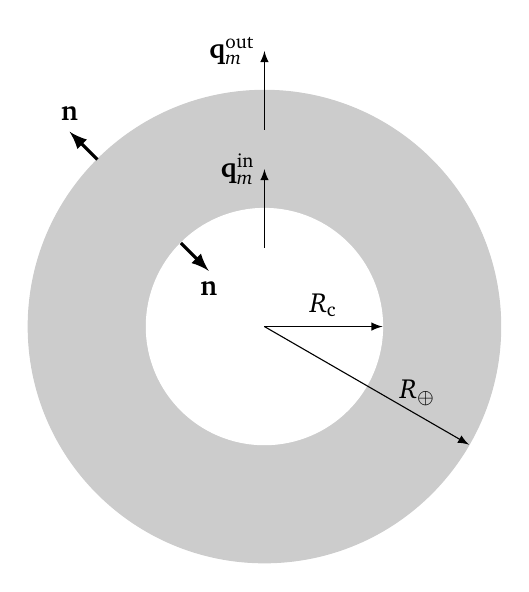
\begin{tikzpicture}
       \draw[dashed,white] (0,-3) -- (0,3.5);
       \filldraw[black!20!white] (0,0) circle [radius=3cm];
       \filldraw[white] (0,0) circle [radius=1.5cm];
       \draw[->] (0,0) -- node[midway,above]{$R_{\text{c}}$}(0:1.5cm);
       \draw[->] (0,0) --  node[near end,above]{$R_{\oplus}$}(-30:3cm);
       \draw[->] (90:1cm) -- (90:2cm) node[left]{$\mathbf{q}^{\text{in}}_m$};
       \draw[->] (90:2.5cm) -- (90:3.5cm) node[left]{$\mathbf{q}^{\text{out}}_m$};
       \draw[very thick,->] (135:3cm) -- (135:3.5cm) node[above]{$\mathbf{n}$};
       \draw[very thick,<-] (135:1cm)node[below]{$\mathbf{n}$} -- (135:1.5cm);
      \end{tikzpicture}
      \caption{Heat flow through inner and outer surfaces of the mantle.}
      \label{fig:flujo_manto}
      \end{subfigure}
      \caption{\label{fig:Earth_interior} Schematics of the Earth's interior structure. Heat flow through the core surface (\subref{fig:flujo_nucleo}) and the inner and outer surfaces of the mantle (\subref{fig:flujo_manto}).}
\end{figure*}

Both the thermal evolution of the core and the mantle are obtained from the energy balance within each layer. Thus, the time evolution of the average internal temperatures of the mantle and core are determined by the balance between the incoming and outgoing heat flux, heat sources and sinks. Among the energy sources are considered radiative decay, both in the mantle and in the core, and the aforementioned tidal interaction, which is assumed to be uniformly distributed in the mantle only. The energy sinks of the mantle are the heat that propagates by convection from the core to the surface and the heat absorbed or released upon melting or solidification of the material that composes the mantle.

\section{Theoretical background\label{sec:theory}}

Let us begin from first principles. Both, the core and mantle, are considered as two separated systems in contact. The thermal states of each of them is characterized by their internal energy, $U$. Since temperatures within Earth's core and mantle are considered to vary with time, then their internal energies will also be time-dependant. The time evolution of $U$ can be tracked by the continuity equation:
\begin{equation}
      \label{ec:Ucontinuity}
      \fdiff{U}{t} + \oiint_S \vec{q} \cdot \text{d} \vec{S} = \fdiff{U_\text{gen}}{t},
\end{equation} where $t$ is time, $\vec{q}$ is the energy flux, which is integrated over a closed surface $S$, and the the term on the right hand side of Eq.~\eqref{ec:Ucontinuity} is the time rate at which the internal energy is generated by sources inside the surface. 

Now, let us rewrite Eq.~\eqref{ec:Ucontinuity} in a more convenient form. To this end, we will consider the first principle of thermodynamics, which relates the change of internal energy ($\Delta U$), the amount of heat exchanged ($Q$), and work ($W$) as:
\begin{equation}
      \label{ec:first_pple}
      \Delta U = Q - W.
\end{equation} Work is related to volume change of the considered system. However, we assume that the volume of both the core and the mantle are fixed, then $W = 0$, and:
\begin{equation}
      \label{ec:first_pple_UQ}
      \Delta U = Q,
\end{equation} that is, the internal energy changes because of exchange of heat between core and mantle, and between mantle and external space. Thus, Eq.~\eqref{ec:Ucontinuity} is rewritten as:
\begin{equation}
      \label{ec:Qcontinuity}
      \fdiff{Q}{t} + \oiint_S \vec{q} \cdot \text{d} \vec{S} = \fdiff{Q_\text{gen}}{t},
\end{equation} where $\vec{q}$ can now formally be identified as the heat flux. Let us consider first the expression of the amount of heat exchanged. For both the core and the mantle we will assume that the heat transferred produces a change in the temperatures ($\Delta T$) and partial melting. Thus, $Q$ is given by:
\begin{equation}
      \label{ec:Qgral}
      Q = M \, c \, \Delta T + L \, M_\text{melt},
\end{equation} where $M$ is the mass, $c$ is the specific heat, $L$ is the latent heat, and $M_\text{melt}$ is the mass of molten or solidified material. Like the volume, the masses of the core and mantle are also assumed constant as well as their physical parameter such as the specific and latent heat. Thus, the rate of change of exchanged heat is associated to changes in temperatures and mass of molten materials. Then, we have:
\begin{equation}
      \label{ec:dQdtgral}
      \fdiff{Q}{t} = M \, c \, \fdiff{T}{t} + L \, \fdiff{M_\text{melt}}{t}.
\end{equation} As we will be explained later, temperature varies within both mantle and core and we will assume that their internal temperatures are function of time and depth (or distance from Earth center, $r$). Since Eq.~\eqref{ec:dQdtgral} is valid for the core and mantle each of them considered as a whole, then the symbol $T$ actually stands for the mean temperature of each layer.

Let us consider now the second term on the left hand side of Eq.~\eqref{ec:Qcontinuity}. In order to compute the surface integral, the core and the mantle need to be considered separately. First of all, in both cases the heat is assumed to flow radially from the Earth's center to its surface. Thus, the heat flux can be expressed as $\vec{q} (t) = q (t) \, \hat{\vec{r}}$, where $\hat{\vec{r}}$ is a unit vector pointing outwards the Earth in radial direction. In addition, the surface element $\text{d} \vec{S}$ can be rewritten as $\text{d} \vec{S} = \vec{n} \, \text{d}S$, where $\vec{n}$ is an unit vector normal to each limiting surface. So, in general, we have that $\vec{q} (t) \cdot \text{d} \, \vec{S} = q (t) \, \text{d}S \left(\hat{\vec{r}} \cdot \vec{n}\right) = \pm q (t) \, \text{d}S$, depending on whether unit vectors $\vec{n}$ and $\hat{\vec{r}}$ have the same or opposite direction. For the core we have that $\vec{q}_c^\text{out} (t) \cdot \text{d} \, \vec{S} = q_c^\text{out} (t) \, \text{d}S$, because unit vectors $\vec{n}$ and $\hat{\vec{r}}$ have the same direction, as can be noted from Fig.~\ref{fig:flujo_nucleo}. In consequence:
\begin{equation}
      \label{ec:oint_core}
      \oiint_{S_c} \vec{q}_c^\text{out} \cdot \text{d} \vec{S} = \oiint_{S_c} q_c^\text{out} (t) \, \text{d}S = q_c^\text{out} (t) \oiint_{S_c} \text{d}S = q_c^\text{out} (t) \, A_c
\end{equation} where $S_c$ indicates that the integration is performed over the core's surface and $A_c$ is the surface area of the core. In the case of the mantle, the surface integral must be divided into two parts, one Corresponding to the inner limiting surface and the other to the outer limiting surface:
\begin{equation}
      \label{ec:oint_mantle}
      \begin{split}
            \oiint_{S_m} \vec{q}_m^\text{out} \cdot \text{d} \vec{S} &= \oiint_{S_m^\text{inner}} \vec{q}_m^\text{in} \cdot \text{d} \vec{S} + \oiint_{S_m^\text{outer}} \vec{q}_m^\text{out} \cdot \text{d} \vec{S} \\
            &= \oiint_{S_{m}^\text{inner}} q_m^\text{in} (t) \, \text{d}S
      \end{split}
\end{equation} The computation of the second integral on the right hand side of Eq.~\eqref{ec:oint_mantle} is totally analogous to the case of the core. Thus:
\begin{equation}
      \label{ec:oint_mantle_outer}
      \oiint_{S_m^\text{outer}} \vec{q}_m^\text{out} \cdot \text{d} \vec{S} = \oiint_{S_m^\text{outer}} q_m^\text{out} (t) \, \text{d}S = q_m^\text{out} (t) \, A_\oplus,
\end{equation} where $A_\oplus$ is the surface area of the Earth. As for the first integral on the right hand side of Eq.~\eqref{ec:oint_mantle}, we have to take into account, on one hand, that the dot product is negative because $\hat{\vec{r}}$ and $\vec{n}$ have opposite directions and, on the other hand, that the inner surface area of the mantle is equal to the core's surface area, i.e. $S_{m}^\text{inner} = S_c$. Then:
\begin{equation}
      \label{ec_oint_mantle_inner}
      \oiint_{S_m^\text{inner}} \vec{q}_m^\text{in} \cdot \text{d} \vec{S} = \oiint_{S_m^\text{inner}} q_m^\text{in} (t) \, \text{d}S = q_m^\text{in} (t) \, A_c.
\end{equation} Moreover, for continuity reasons, and because Earth's core and mantle are in contact with each other, we have that $q_m^\text{in} (t) = q_c^\text{out} (t) = q_\textsc{cmb} (t)$.

Lastly, as we pointed out before, we assume that radioactive decay is a heat source for both the core and the mantle, while tidal heating is present only in the latter. Thus, for the core we have that
\begin{equation}
      \label{ec:dQgendt_core}
      \fdiff{Q_\text{gen}}{t} = \dot{Q}_\text{rad,c},
\end{equation} and for the mantle:
\begin{equation}
      \label{ec:mantle}
      \fdiff{Q_\text{gen}}{t} = \dot{Q}_\text{rad,m} + \dot{Q}_\text{tidal}.
\end{equation}

Then, putting everything together we arrive to the equation governing the thermal evolution of both the core and the mantle:
\begin{align}
      M_c \, c_c \, \fdiff{\valmed{T}_c}{t} + \left(L_c + E_G\right) \, \fdiff{M_\text{ic}}{t} + \dot{Q}_\textsc{cmb} (t) &= \dot{Q}_\text{rad,c} (t) \label{ec:dTmdt_core_gral} \\
      M_m \, c_m \, \fdiff{\valmed{T}_m}{t} + L_m \, \fdiff{M_\text{melt}}{t} - \dot{Q}_\textsc{cmb} (t) + \dot{Q}_\text{conv} (t) &= \dot{Q}_\text{rad,m} (t) + \dot{Q}_\text{tidal} (t), \label{ec:dTmdt_mantle_gral}
\end{align} where the subscripts $c$ and $m$ refers to quantities related to the core and mantle, respectively, $\valmed{T}_i$ (with $i=c,m$) denotes the average temperature of each layer, $\dot{Q}_\textsc{cmb} (t) = q_\textsc{cmb} (t) \, A_c$ and $\dot{Q}_\text{conv} = q_m^\text{out} \, A_\oplus$.

The second term on the left hand side of both Eq.~\eqref{ec:dTmdt_core_gral} and Eq.~\eqref{ec:dTmdt_mantle_gral} are slightly different from that of Eq.~\eqref{ec:dQdtgral} because melting or solidification process in the core and the mantle are different from each other. While the mass of molten material in the mantle, denoted by $M_\text{melt}$, is concentrated in a zone called asthenosphere, which is near the Earth's surface, we assume that the core is completely molten at the beginning of the Earth's history and that solidified core materials precipitate to Earth's center as it cools down forming a solid inner core. Thus, the mass of solidified material within the core is equal to the inner core mass ($M_\text{ic}$). In addition we take into account the gravitational energy release upon solidification of core materials through the parameter $E_G$, which is assumed constant.

In the following subsections, the expressions of the heat fluxes, heat sources, and time rates of melt mass in the mantle and of the inner core mass will be given.

\subsection{Expression of the heat fluxes}

On geological timescales, the dominant heat transport mechanism is convection. The vigor of convection can be measured by the Rayleigh number (Ra). In the case of a fluid limited by two horizontal surfaces and heated from below, analog to Earth's conditions, the Rayleigh number is given by:
\begin{equation}
      \label{ec:Rayleigh_num_def}
      \text{Ra} = \frac{\rho \, \alpha \, g \, \Delta T \, L^3}{\kappa \, \eta},
\end{equation} where $\rho$, $\alpha$, $\kappa$ and $\eta$ are the fluid's density, volumetric expansion coefficient, thermal diffusivity, and dynamical viscosity, respectively, while $\Delta T$ is the temperature jump across the layer of thickness $L$. If Rayleigh number is above some threshold, called the critical Rayleigh number ($\text{Ra}_\text{cr}$), then heat is transported by convection and if it is blow that threshold, then heat is transferred by conduction.

\section{Model implementation\label{sec:model}}

\bibliographystyle{aa}
\bibliography{refs}{}

\end{document}